\documentclass{standalone}
\usepackage{tikz}
\usetikzlibrary{patterns, positioning}


\begin{document}
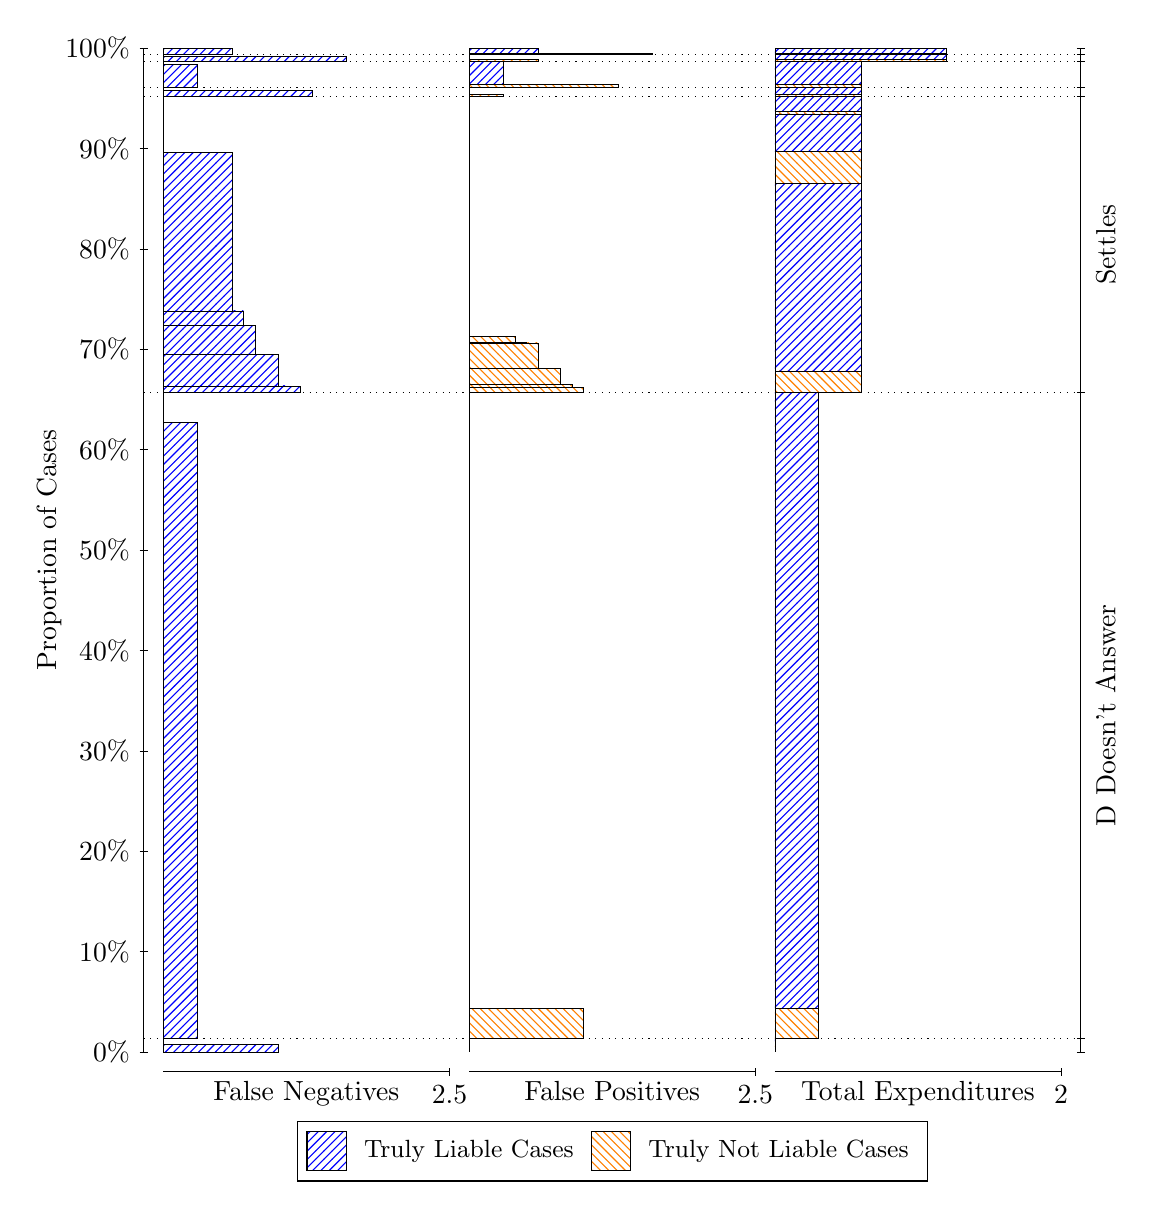
\begin{tikzpicture}
\draw[black, very thin] (1.5,1.75) -- (1.5,14.5);
\node[rotate=90, text=black, anchor=center] at (0.3, 8.125) {Proportion of Cases};
\draw[black, very thin] (1.45,1.75) -- (1.55,1.75);
\node[text=black, anchor=east] at (1.45, 1.75) {0\%};
\draw[black, very thin] (1.45,3.025) -- (1.55,3.025);
\node[text=black, anchor=east] at (1.45, 3.025) {10\%};
\draw[black, very thin] (1.45,4.3) -- (1.55,4.3);
\node[text=black, anchor=east] at (1.45, 4.3) {20\%};
\draw[black, very thin] (1.45,5.575) -- (1.55,5.575);
\node[text=black, anchor=east] at (1.45, 5.575) {30\%};
\draw[black, very thin] (1.45,6.85) -- (1.55,6.85);
\node[text=black, anchor=east] at (1.45, 6.85) {40\%};
\draw[black, very thin] (1.45,8.125) -- (1.55,8.125);
\node[text=black, anchor=east] at (1.45, 8.125) {50\%};
\draw[black, very thin] (1.45,9.4) -- (1.55,9.4);
\node[text=black, anchor=east] at (1.45, 9.4) {60\%};
\draw[black, very thin] (1.45,10.675) -- (1.55,10.675);
\node[text=black, anchor=east] at (1.45, 10.675) {70\%};
\draw[black, very thin] (1.45,11.95) -- (1.55,11.95);
\node[text=black, anchor=east] at (1.45, 11.95) {80\%};
\draw[black, very thin] (1.45,13.225) -- (1.55,13.225);
\node[text=black, anchor=east] at (1.45, 13.225) {90\%};
\draw[black, very thin] (1.45,14.5) -- (1.55,14.5);
\node[text=black, anchor=east] at (1.45, 14.5) {100\%};

\draw[black, very thin] (13.4,1.75) -- (13.4,14.5);
\draw[black, very thin] (13.35,1.75) -- (13.45,1.75);
\node[anchor=west] at (13.35, 1.75) {};
\draw[black, very thin] (13.35,1.9259) -- (13.45,1.9259);
\node[anchor=west] at (13.35, 1.9259) {};
\draw[black, very thin] (13.35,10.125) -- (13.45,10.125);
\node[anchor=west] at (13.35, 10.125) {};
\draw[black, very thin] (13.35,13.881) -- (13.45,13.881);
\node[anchor=west] at (13.35, 13.881) {};
\draw[black, very thin] (13.35,13.997) -- (13.45,13.997);
\node[anchor=west] at (13.35, 13.997) {};
\draw[black, very thin] (13.35,14.331) -- (13.45,14.331);
\node[anchor=west] at (13.35, 14.331) {};
\draw[black, very thin] (13.35,14.422) -- (13.45,14.422);
\node[anchor=west] at (13.35, 14.422) {};
\draw[black, very thin] (13.35,14.5) -- (13.45,14.5);
\node[anchor=west] at (13.35, 14.5) {};

\draw[black, very thin, pattern color=blue, pattern=north east lines] (1.75,1.75) rectangle (3.2033,1.847);
\draw[black, very thin, pattern color=orange, pattern=north west lines] (1.75,1.847) rectangle (1.75,1.9259);
\draw[black, very thin, pattern color=blue, pattern=north east lines] (1.75,1.9259) rectangle (2.186,9.7447);
\draw[black, very thin, pattern color=orange, pattern=north west lines] (1.75,9.7447) rectangle (1.75,10.125);
\draw[black, very thin, pattern color=blue, pattern=north east lines] (1.75,10.125) rectangle (3.494,10.205);
\draw[black, very thin, pattern color=blue, pattern=north east lines] (1.75,10.205) rectangle (3.3487,10.21);
\draw[black, very thin, pattern color=blue, pattern=north east lines] (1.75,10.21) rectangle (3.2033,10.605);
\draw[black, very thin, pattern color=blue, pattern=north east lines] (1.75,10.605) rectangle (2.9127,10.977);
\draw[black, very thin, pattern color=blue, pattern=north east lines] (1.75,10.977) rectangle (2.7673,11.161);
\draw[black, very thin, pattern color=blue, pattern=north east lines] (1.75,11.161) rectangle (2.622,13.172);
\draw[black, very thin, pattern color=orange, pattern=north west lines] (1.75,13.172) rectangle (1.75,13.881);
\draw[black, very thin, pattern color=blue, pattern=north east lines] (1.75,13.881) rectangle (3.6393,13.962);
\draw[black, very thin, pattern color=orange, pattern=north west lines] (1.75,13.962) rectangle (1.75,13.997);
\draw[black, very thin, pattern color=blue, pattern=north east lines] (1.75,13.997) rectangle (2.186,14.293);
\draw[black, very thin, pattern color=orange, pattern=north west lines] (1.75,14.293) rectangle (1.75,14.331);
\draw[black, very thin, pattern color=blue, pattern=north east lines] (1.75,14.331) rectangle (4.0753,14.396);
\draw[black, very thin, pattern color=orange, pattern=north west lines] (1.75,14.396) rectangle (1.75,14.422);
\draw[black, very thin, pattern color=blue, pattern=north east lines] (1.75,14.422) rectangle (2.622,14.493);
\draw[black, very thin, pattern color=orange, pattern=north west lines] (1.75,14.493) rectangle (1.75,14.5);
\draw[black, very thin, pattern color=orange, pattern=north west lines] (5.6333,1.75) rectangle (5.6333,1.8289);
\draw[black, very thin, pattern color=blue, pattern=north east lines] (5.6333,1.8289) rectangle (5.6333,1.9259);
\draw[black, very thin, pattern color=orange, pattern=north west lines] (5.6333,1.9259) rectangle (7.0867,2.3062);
\draw[black, very thin, pattern color=blue, pattern=north east lines] (5.6333,2.3062) rectangle (5.6333,10.125);
\draw[black, very thin, pattern color=orange, pattern=north west lines] (5.6333,10.125) rectangle (7.0867,10.191);
\draw[black, very thin, pattern color=orange, pattern=north west lines] (5.6333,10.191) rectangle (6.9413,10.224);
\draw[black, very thin, pattern color=orange, pattern=north west lines] (5.6333,10.224) rectangle (6.796,10.434);
\draw[black, very thin, pattern color=orange, pattern=north west lines] (5.6333,10.434) rectangle (6.5053,10.756);
\draw[black, very thin, pattern color=orange, pattern=north west lines] (5.6333,10.756) rectangle (6.36,10.76);
\draw[black, very thin, pattern color=orange, pattern=north west lines] (5.6333,10.76) rectangle (6.2147,10.835);
\draw[black, very thin, pattern color=blue, pattern=north east lines] (5.6333,10.835) rectangle (5.6333,13.881);
\draw[black, very thin, pattern color=orange, pattern=north west lines] (5.6333,13.881) rectangle (6.0693,13.916);
\draw[black, very thin, pattern color=blue, pattern=north east lines] (5.6333,13.916) rectangle (5.6333,13.997);
\draw[black, very thin, pattern color=orange, pattern=north west lines] (5.6333,13.997) rectangle (7.5227,14.035);
\draw[black, very thin, pattern color=blue, pattern=north east lines] (5.6333,14.035) rectangle (6.0693,14.331);
\draw[black, very thin, pattern color=orange, pattern=north west lines] (5.6333,14.331) rectangle (6.5053,14.357);
\draw[black, very thin, pattern color=blue, pattern=north east lines] (5.6333,14.357) rectangle (5.6333,14.422);
\draw[black, very thin, pattern color=orange, pattern=north west lines] (5.6333,14.422) rectangle (7.9587,14.43);
\draw[black, very thin, pattern color=blue, pattern=north east lines] (5.6333,14.43) rectangle (6.5053,14.5);
\draw[black, very thin, pattern color=orange, pattern=north west lines] (9.5167,1.75) rectangle (9.5167,1.8289);
\draw[black, very thin, pattern color=blue, pattern=north east lines] (9.5167,1.8289) rectangle (9.5167,1.9259);
\draw[black, very thin, pattern color=orange, pattern=north west lines] (9.5167,1.9259) rectangle (10.062,2.3062);
\draw[black, very thin, pattern color=blue, pattern=north east lines] (9.5167,2.3062) rectangle (10.062,10.125);
\draw[black, very thin, pattern color=orange, pattern=north west lines] (9.5167,10.125) rectangle (10.607,10.401);
\draw[black, very thin, pattern color=blue, pattern=north east lines] (9.5167,10.401) rectangle (10.607,12.783);
\draw[black, very thin, pattern color=orange, pattern=north west lines] (9.5167,12.783) rectangle (10.607,13.184);
\draw[black, very thin, pattern color=blue, pattern=north east lines] (9.5167,13.184) rectangle (10.607,13.664);
\draw[black, very thin, pattern color=orange, pattern=north west lines] (9.5167,13.664) rectangle (10.607,13.697);
\draw[black, very thin, pattern color=blue, pattern=north east lines] (9.5167,13.697) rectangle (10.607,13.881);
\draw[black, very thin, pattern color=orange, pattern=north west lines] (9.5167,13.881) rectangle (10.607,13.916);
\draw[black, very thin, pattern color=blue, pattern=north east lines] (9.5167,13.916) rectangle (10.607,13.997);
\draw[black, very thin, pattern color=orange, pattern=north west lines] (9.5167,13.997) rectangle (10.607,14.035);
\draw[black, very thin, pattern color=blue, pattern=north east lines] (9.5167,14.035) rectangle (10.607,14.331);
\draw[black, very thin, pattern color=orange, pattern=north west lines] (9.5167,14.331) rectangle (11.697,14.357);
\draw[black, very thin, pattern color=blue, pattern=north east lines] (9.5167,14.357) rectangle (11.697,14.422);
\draw[black, very thin, pattern color=orange, pattern=north west lines] (9.5167,14.422) rectangle (11.697,14.43);
\draw[black, very thin, pattern color=blue, pattern=north east lines] (9.5167,14.43) rectangle (11.697,14.5);
\draw[black, dotted] (1.5,1.9259) -- (13.4,1.9259);
\draw[black, dotted] (1.5,10.125) -- (13.4,10.125);
\draw[black, dotted] (1.5,13.881) -- (13.4,13.881);
\draw[black, dotted] (1.5,13.997) -- (13.4,13.997);
\draw[black, dotted] (1.5,14.331) -- (13.4,14.331);
\draw[black, dotted] (1.5,14.422) -- (13.4,14.422);
\draw[black, very thin] (1.75,1.5) -- (5.3833,1.5);
\node[text=black, anchor=north] at (3.5667, 1.5) {False Negatives};
\draw[black, very thin] (5.3833,1.45) -- (5.3833,1.55);
\node[text=black, anchor=north] at (5.3833, 1.45) {2.5};

\draw[black, very thin] (5.6333,1.5) -- (9.2667,1.5);
\node[text=black, anchor=north] at (7.45, 1.5) {False Positives};
\draw[black, very thin] (9.2667,1.45) -- (9.2667,1.55);
\node[text=black, anchor=north] at (9.2667, 1.45) {2.5};

\draw[black, very thin] (9.5167,1.5) -- (13.15,1.5);
\node[text=black, anchor=north] at (11.333, 1.5) {Total Expenditures};
\draw[black, very thin] (13.15,1.45) -- (13.15,1.55);
\node[text=black, anchor=north] at (13.15, 1.45) {2};


\node[text=black, centered, rotate=90] at (13.72, 6.0254) {D Doesn't Answer};
\node[text=black, centered, rotate=90] at (13.72, 12.003) {Settles};





\draw (7.449999999999999,1.5) node[draw=none] (baseCoordinate) {};
\begin{scope}[align=center]
        \matrix[scale=0.5, draw=black, below=0.5cm of baseCoordinate, nodes={draw}, column sep=0.1cm]{
            \node[rectangle, draw, minimum width=0.5cm, minimum height=0.5cm, pattern color=blue, pattern=north east lines] {}; &
            \node[draw=none, font=\small, text=black] (B) {Truly Liable Cases}; &
            \node[rectangle, draw, minimum width=0.5cm, minimum height=0.5cm, pattern color=orange, pattern=north west lines] {}; &
            \node[draw=none, font=\small, text=black] (B) {Truly Not Liable Cases}; \\
            };
\end{scope}

\end{tikzpicture}
\end{document}